%!TEX root = ../thesis.tex
%*******************************************************************************
%****************************** Second Chapter *********************************
%*******************************************************************************

\chapter{Methods}

\ifpdf
    \graphicspath{{Chapter2/Figs/Raster/}{Chapter2/Figs/PDF/}{Chapter2/Figs/}{Figs}}
\else
    \graphicspath{{Chapter2/Figs/Vector/}{Chapter2/Figs/}{Figs}}
\fi

\section{A general model for the dynamics of alternative
 sigma factors}
% originally the equations are listed under a subsection
% related to low copy numbers. Now it is moved under the
% main title, but the tag is retained.
\label{sec:low_CN}

To further investigate the relationship between sigma factor dynamics
and the circuit 
% here I was trying to link to phenotypic variations, but seems weird
structure, i.e. how the molecules in a sigma factor network interact
with each other,
I formalized a simplified but mechanistic model to describe the system.
The model is then simulated using the Gillespie algorithm to ensure
accuracy under low copy number of molecules.
The various dynamical behaviours produced by the model may not only
serve as a theoretical explanation of the observed dynamics,
but also may give insights into other potential behaviours
(e.g. Figure~\ref{fig:different_behaviours}).
From there, I further discussed how bistability may arise without
binding cooperativity in the circuit,
a phenomenon that was not clearly accounted for in previous studies.
To accommodate the Gillespie algorithm, the system is described 
as master equations
(adopted from Torkel Loman's unpublished work):

\begin{equation}    % to give only one label to equations
\label{eqn:master_eqn}
\begin{gathered}    % for some reason, gather does not work here...
    \sigma\quad\xrightarrow{\quad \frac{\beta}{\tau_S}\left(
        v_0 + v_H\right)\quad}\quad\sigma + 1\\
    \sigma\quad\xrightarrow{\quad \frac{1}{\tau_S}\sigma \quad}
        \quad\sigma - 1\\
    A\quad\xrightarrow{\quad \frac{\beta}{\tau_A}\left(
        v_0 + v_H\right)\quad}\quad A + 1\\
    A\quad\xrightarrow{\quad \frac{1}{\tau_A}A \quad}\quad A - 1
\end{gathered}
\end{equation}

The state of the system is determined by two variables:
the copy number of the sigma factors ($\sigma$) and the copy number
of anti-sigma factors ($A$).
The probability of the transition between adjacent states
(i.e. the production or degradation of a single sigma factor/anti-sigma
factor) is a function of the current $\sigma$ and $A$.
The corresponding transition probabilities are shown above the
arrows, where $v_0$ is the basal expression rate (a constant)
and $v_H(\sigma, A)$ is the primary expression rate.
Here, $v_H(\sigma, A)$ is derived from binding kinetics and
reflects the circuit structure.
Other parameters include $\beta$, the maximum expression rate,
and $\tau_S$ and $\tau_A$, which are respectively the (average)
molecular lifetime of $\sigma$ and $A$.
The primary expression rate $v_H$ is written as:

\begin{align}
    v_H = \frac{\sigma/K_S}{\sigma/K_S + (A/K_D)^n + 1}
\end{align}

Where $K_S$ and $K_D$ are two different dissociation constants which
reflect the binding equilibriums of the system.
$n$ here is the apparent binding cooperativity, which is an indicator
of ultrasensitivity.
However, as mentioned previously in Section~
\ref{sec:biochemical_ultrasensitivity}, many sigma factor circuits
do not have known binding cooperativity, but whose observed
dynamical behaviours are suggested to rely on ultrasensitivity.
I will revisit this parameter $n$ later.

Though may be obscured by the formalization required by the 
Gillespie algorithm, the model (Eq.~\ref{eqn:master_eqn}) generally
depends on only two major assumptions, namely

\begin{itemize}
    \item The circuit only contains two protein species: the sigma
    factor ($\sigma$) and the anti-sigma factor ($A$).
    \item The sigma factor is under positive autoregulation, but
    also under negative feedback through the anti-sigma factor.
\end{itemize}

Besides the well-studied $\sigma^B$ factor, other sigma factors
such as $\sigma^D$, $\sigma^W$, and $\sigma^X$ 
\cite{haldenwang95, huang98, hsueh11} can all be 
abstracted in a such way in line with these assumptions.
Other assumptions include that the binding events are much
faster than transcriptions so that binding is considered to be
at equilibrium, and, similarly, that translation is much 
faster than translation, so that the expression rate is the
combination of the two, etc.


%%%%%%%%%%%%%%%%%%%%%%%%
% Old writings
%%%%%%%%%%%%%%%%%%%%%%%%
% Here I propose a general model to explain the spectrum of 
% dynamical behaviours, e.g. stochastic pulsing \cite{locke11,cabeen17},
% transient pulsing and sustained activation \cite{cabeen17}
% of the bacterial alternative sigma factors in the species 
% \textit{B. subtilis}.
% It also serves as the foundation of the sigma factor competition
% model (Section~\ref{sec:sigma_competition_model}).
% The model is based on the general topology that is 
% shared by multiple alternative sigma factor networks
% including $\sigma^D$, $\sigma^W$, $\sigma^X$, etc
% \cite{haldenwang95, huang98, hsueh11}, namely

% \begin{itemize}
%     \item The sigma factor is under positive autoregulation, i.e.,
% the sigma factor activates its own expression.
%     \item An anti-sigma factor is co-expressed with the sigma factor as its
% inhibitor, forming a negative feedback loop.
% \end{itemize}

% I formalize a minimal mechanistic model based on these network topologies.
% Without loss of generality, the following model reflects the $\sigma^B$
% regulatory network but is applicable to other alternative sigma factors.

\subsection{Sigma-anti-sigma binding kinetics}

The primary expression rate, $v_H$, which is expressed as a Hill function
(thus the denotation), is derived from the binding kinetics between the
sigma factor and the anti-sigma factor,
and that between the RNAP holoenzyme (comprising the sigma factor) and the promoter.
Notice that $v_H$ is shared by the production step of both the sigma factor
and the anti-sigma factor, since they are located in the same operon.
%%
First, the promoter of the operon including the gene that encodes the sigma factor
is transcribed by the RNA polymerase (RNAP) holoenzyme comprising 
the sigma factor itself.
The relative transcription rate (denoted by $v_H$) to the maximal rate 
is modelled by Hill kinetics with ultrasensitivity encoded in $n$:

\begin{align}
    \label{eqn:v_hill}
    v_H = \frac{\sigma_f^n}{K_S^n + \sigma_f^n}
\end{align}

where $\sigma_f$ is the abundance of the unbound sigma factors, as
the anti-sigma factor (denoted by $A$), competes the binding of 
sigma factors with RNAP cores.
$K_S$ is the dissociation constant between the RNAP holoenzyme and the promoter.
$n$ is the Hill coefficient, which represents the apparent binding cooperativity.

Second, the anti-sigma factor ($A$) sequesters the sigma factor ($\sigma$)
from the RNAP core by binding to it and forming a complex (denoted by $A\sigma$).
As the binding is on a faster time scale than transcription,
the binding dynamics can be considered at steady-state in
transcriptional regulation.
The binding dynamics is governed by 

\begin{gather}
    \label{eqn:W_binding}
    K_D = \frac{A_f\cdot \sigma_f}{A\sigma}\\
    \label{eqn:total_sigma}
    \sigma = \sigma_f + A\sigma
\end{gather}

where $\sigma$ is the total abundance of sigma factors
and $A_f$ is the amount of unbound anti-sigma factors.
$K_D$ is the dissociation constant of sigma-anti-sigma factor binding.
Together, Eq.~\ref{eqn:W_binding} and Eq.~\ref{eqn:total_sigma}
bridges the abundance of free sigma factors and 
the total number of sigma factors as

\begin{align}
    \label{eqn:sigma_f}
    \sigma_f = \frac{K_D}{K_D + A_f}\sigma
\end{align}

i.e. the binding is subject to Michaelis-Menten kinetics,
which, in the general model described here, is considered
as non-cooperative.
Finally, under the assumption that the anti-sigma factor is in excess
to the sigma factor so that $A \approx A_f$,
Eq.~\ref{eqn:v_hill} can be re-written as

\begin{align}
    \label{eqn:v_hill_2}
    v_H = \frac{(\sigma/K_S)^n}{(\sigma/K_S)^n + (A/K_D + 1)^n}
\end{align}

Given Eq.~\ref{eqn:v_hill_2} where ultrasensitivity is derived from
the cooperativity of transcription initiation,
there are other steps in the core sigma factor network that can
potentially contribute to $n$,
e.g., for $\sigma^B$ network, RsbW dimerizes to bind $\sigma^B$, which
is captured by as $\sigma_f = K_D^2/(K_D^2 + A_f^2)\cdot\sigma$.
Generalization leads to an alternative form of Eq.~\ref{eqn:v_hill_2}
where the cooperative binding between sigma factors and anti-sigma factors
solely accounts for the ultrasensitivity.

\begin{align}
    v_H = \frac{\sigma/K_S}{\sigma/K_S + (A/K_D)^n + 1}
\end{align}

\subsection{Activation of the circuit}

Here I take the $\sigma^B$ circuit as an example to explain the model.
Upon exposure to the stressor,
a phosphatase, either RsbQP or RsbTU is released, depending on whether the
environmental stress or energy stress is applied.
This process in turn dephosphorylates the anti-anti-sigma factor RsbV to
its activated form (which the activated from is denoted by $V$).
RsbV competes the binding of RsbW with $\sigma^B$, which releases
$\sigma^B$ and, thus, triggers the stress response.

Similar to Eq.~\ref{eqn:sigma_f}, at steady-state,
the abundance of RsbW free to RsbV binding is captured 
by Michaelis-Menten kinetics

\begin{align}
    \label{eqn:A_f}
    A_f = \frac{K_A}{K_A + V}A
\end{align}

Notice that the $A$ term in Eq.~\ref{eqn:v_hill_2} is essentially the unbound
anti-sigma factor, which, according to Eq.~\ref{eqn:A_f},
is a function of the activated RsbV and 
the total amount of anti-sigma factors.
Substituting Eq.~\ref{eqn:A_f} in to Eq.~\ref{eqn:v_hill_2}, we then have

\begin{align}
    v_H = \frac{(\sigma/K_S)^n}
        {(\sigma/K_S)^n + \left(\frac{A}{(1 + V/K_A)K_D} + 1\right)^n}
\end{align}

Here, I define the apparent sigma-anti-sigma dissociation constant as
$K_D' = (1 + V/K_A)\cdot K_D$, which then keeps the mathematical form
of Eq.~\ref{eqn:v_hill_2} unchanged.
Thus, upon stress, the step-increase in the
abundance of dephosphorylated RsbV is modelled by a step-increase
of the apparent $K_D$.

Admittedly, not every sigma factor circuit includes an anti-anti-sigma factor,
thus the derivations above are not readily applicable to other 
sigma factor circuits.
However, for simplicity, it is still reasonable to model the activation
of the system as a step-change in the parameter $K_D$,
as it may also represent the effect of activation
ignorant of the actual mechanism.



\subsection{Modelling stochastic fluctuation under low copy number}

The alternative σ factors typically exist in low copy number and,
thus, their abundance is subject to stochastic fluctuation.
In \textit{Escherichia coli}, while there can be thousands of housekeeping
$\sigma^{70}$ factor per cell, the number of alternative $\sigma^E$
factor is only about 160 even under stress \cite{collinet00}.


Since noise can be crucial to the pulsing dynamics \cite{park18a},
and that noise is stronger under low copy numbers,
I model the system with the Gillespie algorithm to ensure the 
accuracy of simulation when the molecular abundance is low.
The model expressed in master equations is shown in
Eq~\ref{eqn:master_eqn}.

% I model the system with the exact molecular number of
% the alternative σ factor ($\sigma$) and the anti-sigma factor
% ($A$) as the state variables,
% and the random walk through state-space with jump events
% (based on the unpublished work of Torkel Loman):

% \begin{gather}
%     \sigma\quad\xrightarrow{\quad \frac{\beta}{\tau_S}\left(
%         v_0 + v_H\right)\quad}\quad\sigma + 1\\
%     \sigma\quad\xrightarrow{\quad \frac{1}{\tau_S}\sigma \quad}
%         \quad\sigma - 1\\
%     A\quad\xrightarrow{\quad \frac{\beta}{\tau_A}\left(
%         v_0 + v_H\right)\quad}\quad A + 1\\
%     A\quad\xrightarrow{\quad \frac{1}{\tau_A}A \quad}\quad A - 1
% \end{gather}

% where the relative transcription rate, $v_H$ is given
% by Eq.~\ref{eqn:v_hill_2}.
% The transcription rate is generalized which also 
% accounts for translation.
% $v_0$ is the basal transcription activity and $\beta$ is the maximal
% transcription rate, which determines the steady-state abundance.
% If steady-state is reached, the average abundance of both species
% equals to $\beta v_H$ (ignoring basal transcription),
% i.e. $\langle \sigma \rangle = \langle A \rangle$.
% The same primary transcription rate is shared between $\sigma$ and $A$
% since they are co-expressed in the same operon.

The parameters used in the model or its derivation are summarized
in Table~\ref{tab:general_model_paras}.

\begin{table}[ht]
    \centering
    \begin{tabular}{|c|p{3.5in}|c|}\hline
        Parameter & Description & Units\\\hline
        $K_S$ & Dissociation constant between the sigma factor-
        RNAP core complex and the promoter & Molecules per cell\\
        $K_D$ & Dissociation constant between the sigma factor
        and the anti-sigma factor & Molecules per cell\\
        $K_A$ & Dissociation constant between the anti-sigma factor
        and the anti-anti-sigma factor & Molecules per cell\\
        $\tau_S$ & Average molecular lifetime of the sigma factor &
        Arbitrary units\\
        $\tau_A$ & Average molecular lifetime of the anti-sigma factor &
        Arbitrary units\\
        $\beta$ & Maximal expression rate of the operon containing the sigma
        factor and the anti-sigma factor when fully activated
        & Molecules per cell\\
        $v_0$ & Scaled basal expression rate of the operon & -\\
        $v_H$ & Scaled primary expression rate of the operon & -\\\hline
    \end{tabular}
    \caption[Parameter list of the sigma factor model]
    {\textbf{Parameter list of the sigma factor model}}
    \label{tab:general_model_paras}
\end{table}

\subsection{Nondimensionalization of time}
\label{sec:methods_nondim_time}    % there is a similar section in discussion

Though the chemical species are measured in absolute number of molecules (per cell),
the quantities related with time, such as molecular lifetime and
the reaction rates, are on a relative scale.
The Gillespie algorithm is not dependent on the time scale that one chooses,
which warrants this nondimensionalization of time.
Also to support it, I measured the variation of the copy number of sigma factors
at equilibrium when the system is in the dynamical regime of 
constant expression.
The variation remains the same when changing the absolute unit of time
(but keeping the relative amounts).
To be specific, the average lifetime of the sigma factor is set to 10
units of time for most simulations, while the lifetime of the anti-sigma
factor is 50, being 5 times longer than that of the sigma factor.
This settings ensures a delay in the negative feedback (through the 
anti-sigma factor) relative to the self-activation of the sigma factor.
I suggest that the delay is essential for some behaviours, e.g.,
oscillation. Specifically, oscillation cannot maintain if the lifetime of 
the anti-sigma factor is smaller than that of the sigma factor, i.e.,
if without delay in the negative feedback loop (data not shown).
Though the idea is not fully developed in this thesis,
it may be as interesting a topic as exploring the influence of ultrasensitivity
to ask what is the role of delay in the circuit.


\section{Simulation of the model}

The model is simulated by the Gillespie algorithm, i.e. the
Stochastic Simulation Algorithm \cite{gillespie77},
which generates statistically accurate trajectories of the
jump processes described in Section~\ref{sec:low_CN} as
a Markov process.
The algorithm I used is provided by the Catalyst.jl \cite{catalystjl} package,
which an interface around DifferentialEquations.jl \cite{rackauckas17},
of the Julia language \cite{Julia-2017}.


\section{A sigma factor competition model}
\label{sec:sigma_competition_model}

% "dual" sigma factor model
To explore the emerged dynamics from the competition of different
sigma factors for limited RNAP core enzymes,
I built a model consisting of two sigma factor circuits,
whose biochemical parameters ($n$, $K_S$, $K_D$, etc.) are independent.
%%
For simplicity, the model only focuses on two of the various 
alternative sigma factors (for context, \textit{B. subtilis} has 17 
different alternative sigma factors \cite{park18a}).
%% 
% the actual number of RNAP cores is addressed in either 
% parameters or discussion
The influence of the remaining sigma factors, including the 
housekeeping one, is averaged and reflected by the limited
number of available RNAP cores.
%%
In addition to the model of the core circuit (Section~\ref{sec:low_CN}),
the competition model links the two sigma factors by 
the association to and dissociation from a shared pool of
RNAP cores:

\begin{gather}
    E + \sigma \quad \xrightarrow{\quad k_{on} \quad} \quad E\sigma\\
    E\sigma \quad \xrightarrow{\quad k_{off} \quad} E + \sigma
\end{gather}

Where $E$ is the RNAP core enzyme and $\sigma$ represents
either of the two competing sigma factors.
%%
The reaction rate follows the law of mass reaction (considering
elementary reactions) with the association rate constant $k_{on}$ and
dissociation rate constant $k_{off}$.
%%
The rate constants relate to the equilibrium binding affinity 
(expressed by the dissociation constant $K_{E\sigma}$) by
\cite{john12}

\begin{align}
    \label{eqn:disso_constant_to_rates}
    K_{E\sigma} = \frac{k_{off}}{k_{on}}
\end{align}

The total amount of RNAP cores, captured by $E + E\sigma$
in the model, is essentially the pool of RNAP cores that
are accessible to the two sigma factors here subtracting
the proportion already bound by the housekeeping sigma factor and
other alternative ones.
%%
This value is assumed constant since both the total 
RNAP cores (shared by all sigma factors) and the housekeeping
sigma factors remain relatively constant in different
growth conditions \cite{osterberg11}.
%%
Admittedly, the assumption is impaired by the fluctuating 
amount of other alternative sigma factors, 
which motivates a multi-sigma factor competition model in
future study.


% I put this after the competition model to allow a further 
% explanation of those parameters
\section{Model parameters}

% why we care about the actual values of the parameters
The values of the parameters matter since the behaviour of the system
can change drastically when tuning some of the parameters,
e.g. when changing $n$ that represents ultrasensitivity.
The parameters are of biological significance.
Thus, the validity of the model partially depends on whether
the parameters match actual measurements.
% the general model
For most simulations, $\beta$ is set to 50.
This parameter dictates the equilibrium number of sigma factors
per cell when the expression of sigma factor is activated,
which aligns with the literature value from tens to thousands
\cite{collinet00,mauri14} but is on the fewer side to emphasize
the effects of fluctuations at low copy number.
As mentioned in Section~\ref{sec:methods_nondim_time},
the units of time is arbitrary, but to allow some dynamical behaviours,
e.g. oscillation, the average lifetime of the sigma factor should
be shorter than that of the anti-sigma factor ($\tau_S < \tau_A$).

% now the competition model
In the sigma factor competition model, the dissociation constant
between the sigma factor and the RNAP core ($K_{E\sigma}$) contributes crucially
to the strength of the competition.
A study reports that the constant can range from ~1 to more than 100
molecules per cell (in typical bacteria, \SI{1}{\nano\Molar} converts
to approximately 0.8 molecules per cell),
which sets the range of the simulation in this thesis.
RNAP holoenzyme forming kinetics, characterized by the rates
$k_{on}$ and $k_{off}$ are also ruled by $K_{E\sigma}$ through
Eq~\ref{eqn:disso_constant_to_rates} (more discussed in
Section~\ref{sec:discussion_parameters}).
Finally, it is important to point out that given the degree of
simplicity and some presumptions used in the model,
more accurate measurements of the biological system does not
necessarily improve the predictability of the model.
The model is meant to provide insights on how the circuit is 
tuned by several biophysical properties of the molecules.
Thus, it is still important to assess the system under
certain changes and then evaluate the predictions given by this model.


% Notes: the algorithm lies at the core of the thesis
% but is painful to formally write it down.
% partially because it evolves over time and, awkwardly,
% it relies on several hard-coded, even fine-tuned parameters
\section{A classification algorithm for dynamical behaviours}
\label{sec:classification_algorithm}

% goal of the algorithm
To effectively explore how the different behaviours generated by the model
with different parameters,
I developed the automatic classifier.
The classification algorithm described here takes the 
discrete-valued trajectories of a two-species reaction system as
the input and classifies the system as one of
the qualitatively distinct behaviours.
% an overall description of the algorithm
The pre-stress (i.e. pre-perturbation) trajectory is truncated before further analysis.
The classification is done by examining the phase-plane 
(i.e., the $\sigma$-$A$ plane) characteristics.
Since the system written in discrete master equations (Eq. \ref{eqn:master_eqn})
instead of ODEs, I will first reconstruct the flow by estimating
the vector field from the Gillespie-simulated trajectories as described in
Section \ref{sec:reconstruction}.

Inspired by continuous models, I located the "fixed points" of the system
which are the maxima of the density of the trajectories.
Combined with the"flow" across the fluctuation threshold (detailed in Section \ref{sec:detecting_fp}), etc.
and Fourier analysis of the trajectory,
the algorithm determines the type of dynamics by a decision tree
(Figure~\ref{fig:classifier_flowchart}).

\subsection{Reconstructing the vector field from simulation}
\label{sec:reconstruction}

In my algorithm, the reconstructed vector field and the trajectory densities
are important for identifying the fixed points, and thus,
for determining the behaviour types.
%
First, the trajectory density, $I$, is defined at each lattice point 
$(\sigma, A)$ as the number of times that the post-stress trajectory passes
that point.
%
Then, the vector field requires the gradient at each lattice point.
The gradient at point $(\sigma_k, A_k)$ is denoted as 
$(\dot{\sigma}_k, \dot{A}_K)$. It is calculated in a manner similar to
the symmetric derivative at $(\sigma_k, A_k)$ and is averaged
among all the times that the trajectory passes $(\sigma_k, A_k)$.
Formally, the two components of the gradient are

\begin{align}
    \dot{\sigma}_k &= \frac{1}{I(\sigma_k, A_k)}\sum_{t \in T_k}
    \frac{\sigma(t + \Delta t) - \sigma(t - \Delta t)}{2\Delta t}\\
    \dot{A}_k &= \frac{1}{I(\sigma_k, A_k)}\sum_{t \in T_k}
    \frac{A(t + \Delta t) - A(t - \Delta t)}{2\Delta t} \text{,}
\end{align}

where $I(\sigma_k, A_k)$ is the trajectory density at point $(\sigma_k, A_k)$,
$T_k$ is the set of time points where the trajectory passes
$(\sigma_k, A_k)$, 
formally $T_k = \left\{t|\sigma(t) = \sigma_k \;\text{and}\; A(t) = A_k\right\}$,
and $\Delta t$ is the time step of the simulation.

% First, the algorithm recreates the phase-plane paths and the 
% vector field of time-derivatives from the trajectories.
% The intensity ($I$) of phase-plane path of each lattice point on the 
% phase plane is calculated as the total number of times that
% the path passes the point.
% The time-derivative at the point $(\sigma_k, A_k)$ is approximated by

% \begin{align}
%     \dot{\sigma} &= \frac{1}{I(\sigma_k, A_k)}\sum_{t_k}
%     \frac{\sigma(t_k + \Delta t) - \sigma(t_k - \Delta t)}{2\Delta t}\\
%     \dot{A} &= \frac{1}{I(\sigma_k, A_k)}\sum_{t_k}
%     \frac{A(t_k + \Delta t)- A(t_k - \Delta t)}{2\Delta t}
% \end{align}

% where $t_k$ are the time points after exposure to stress which satisfies
% $\sigma(t_k) = \sigma_k \text{and} A(t_k) = A_k$.
% More explicitly, the phase-plane path travels to $(\sigma_k, A_k)$ at time $t_k$.

\subsection{Detection of fixed points and "flows" across the fluctuation thresholds}
\label{sec:detecting_fp}
%
For continuous models e.g. ODEs, if a stable fixed point exists,
trajectories in the \emph{basin of attraction} of the fixed point will eventually
converge to it.
This results in a high trajectory density about the stable fixed point.
The maxima of the density of a Gillespie trajectory plays a similarly important
role to announce the type of dynamics of a discrete model.
For the sake of argument, I will call these maxima as the "fixed points" of
the discrete model.
Notice that the maxima of density do not necessarily behaviour in the way
of stable fixed points of ODEs.
E.g., The Gillespie trajectory in Figure \ref{fig:density_and_vf} behaviours as a homoclinic
connection, a circle solution connecting to a saddle.
Such dynamics allow the phase point to linger around the saddle for a good amount
of time while occasionally visiting the loop, which leads to a maximum at the saddle
(Figure \ref{fig:density_and_vf} B).
We categorize this behaviour as stochastic pulsing, intuitively similar to the firing
of a neuron (see \cite{hesse22} for a model of action potential with homoclinic connections).
%
The classification algorithm relies on identifying the fixed points of the
Gillespie model. Density on the phase plane is defined as the number of times that
the trajectories visit each grid point. The densities are smoothed and
the fixed points are found at the local maxima.

The flow on the phase plane, expressed as a vector field,
is also approximated from the trajectories generated
from the stochastic model. We pay specific attention to the flow on the fluctuation thresholds

\begin{align}
    \sqrt{\sigma_x^2} = \sqrt{\beta/n}
    \label{eqn:fluc_threshold}
\end{align}

Which derives from the fluctuation-dissipation theorem\cite{paulsson05a}

\begin{align}
    \frac{\sigma_x^2}{<x>^2} = \frac{1}{n<x>}
\end{align}

Where $\sigma_x^2$ is the variance of the expression of gene $x$, namely
$\sigma_x^2 = <x^2> - <x>^2$. $n$ is the Hill coefficient.
The mean expression level at steady state $<x>$ is determined by the parameter $\beta$,
which then gives Eqn. \ref{eqn:fluc_threshold}.
Practically, I usually use twice of the theoretical threshold to distinguish
a bona fide equilibrium from excitable dynamics.
The caveats would be that (1) the choice of the fluctuation threshold determines
the type of dynamics on the boundary of two categories, e.g., a dynamics where
the flow settles most of the time but excites only rarely
and (2) the fluctuation-dissipation may not be applicable for out-of-steady-state
systems\cite{chabot07}.
The flow crossing the $\sigma$-axis or the $A$-axis are denoted as the forward flow
$I_{forward}$ or the reverse flow $I_{reverse}$ respectively.
Both of the flows and the existence of "fixed points" are then feed into the 
algorithm to decide the type of dynamics.

\begin{figure}
    \centering
    \begin{subfigure}{0.45\textwidth}
        \centering
        \includegraphics[width=\textwidth]{Figs/2_5_algo_example_traj.pdf}
        \caption{Trajectory}
    \end{subfigure}
    \hfill
    \begin{subfigure}{0.45\textwidth}
        \centering
        \includegraphics[width=\textwidth]{Figs/2_5_algo_example_density.pdf}
        \caption{Density}
    \end{subfigure}
    
    \begin{subfigure}{0.45\textwidth}
        \centering
        \includegraphics[width=\textwidth]{Figs/2_5_algo_example_vf.pdf}
        \caption{Vector field}
    \end{subfigure}
    \caption[Example trajectory of the discrete model, density on the phase plane,
    and reconstructed vector field]
    {Example trajectory of the discrete model, density on the phase plane,
    and reconstructed vector field}
    \label{fig:density_and_vf}
\end{figure}

Finally, Figure~\ref{fig:classifier_flowchart} shows the flowchart
to decide the classification, where
$N_{small}$ is the number of stable fixed points where the abundance
of both species are greater than the threshold $T_{fluc}$,
and similarly, $N_{large}$ is the number of stable fixed points
which the abundance of both species are less than $T_{fluc}$.
$I_{forward}$, or the forward flow, is defined as the sum of 
intensity on the vertical segment from $(T_{fluc}, 0)$ to 
$(T_{fluc}, T_{fluc})$.
Similarly, the reverse flow $I_{reverse}$ is the sum of intensity
on the horizontal segment from $(0, T_{fluc})$ to $(T_{fluc}, T_{fluc})$.



\begin{figure}[ht]
    \centering
    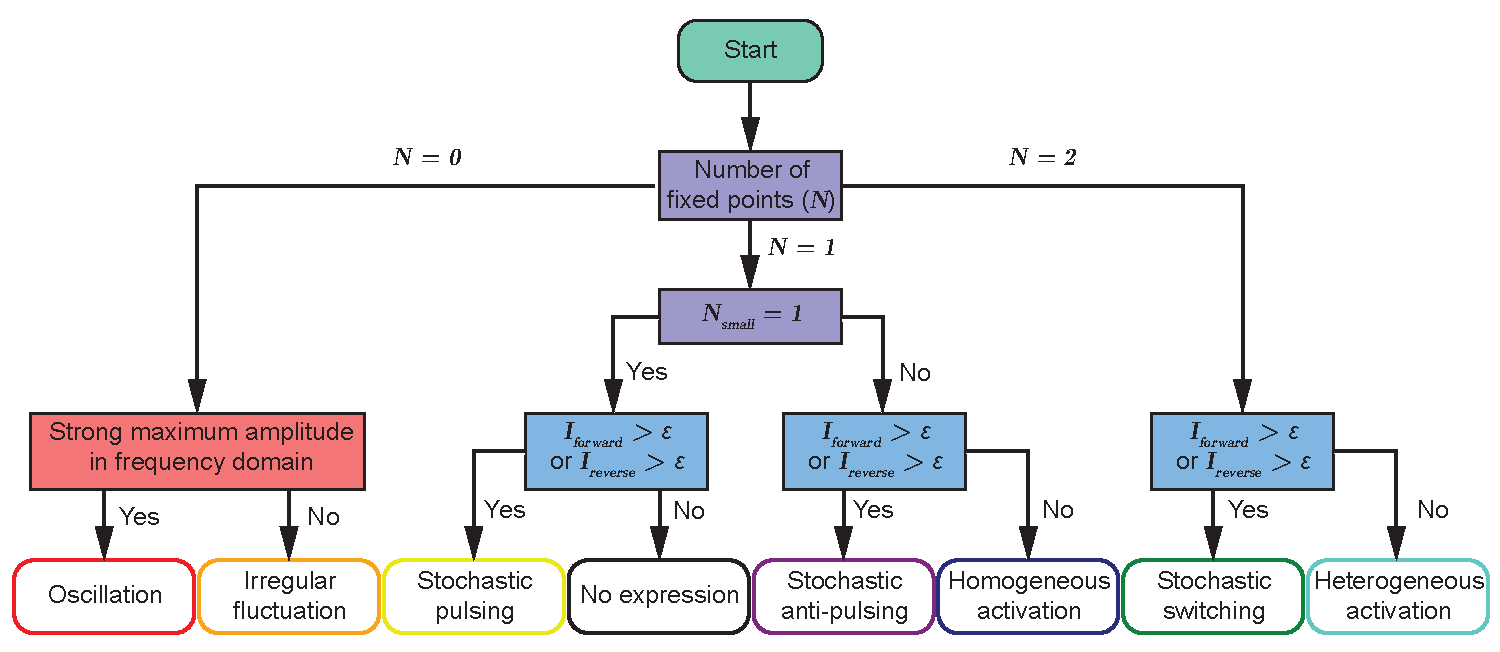
\includegraphics[width=6in]{classifier_flowchart_remake}
    \caption[The decision tree for different behaviour types] {
        \textbf{The decision tree for different behaviour types} lies at
        the core of the classification algorithm. Several phase-plane
        properties are reconstructed from the Gillespie-simulated trajectories.
        The phase-plane properties determine the behaviour types.
        $N$ is the number of fixed points. $N_{small}$ is the number of
        fixed points close to the origin, which are formally the ones below
        the fluctuation threshold.
        $I_{forward}$ and $I_{reverse}$ are respectively the forward and
        reverse flow of the trajectory across the fluctuation threshold.
        $\epsilon$ is a small amount. I used $\epsilon = 1 \times 10^{-4}$
        in the algorithm.
        A strong maximum amplitude is defined as that the maximum amplitude 
        $> 50$ folds of the average of its vicinity.
    }
    \label{fig:classifier_flowchart}
\end{figure}

% I don't have time to develop this section
% admittedly, not a very mature concept, but would be
% interesting/useful to develop it further

% \subsection{Determine the threshold from the level of stochastic fluctuation}

